% Options for packages loaded elsewhere
\PassOptionsToPackage{unicode}{hyperref}
\PassOptionsToPackage{hyphens}{url}
\PassOptionsToPackage{dvipsnames,svgnames,x11names}{xcolor}
%
\documentclass[
  11pt,
]{article}

\usepackage{amsmath,amssymb}
\usepackage{iftex}
\ifPDFTeX
  \usepackage[T1]{fontenc}
  \usepackage[utf8]{inputenc}
  \usepackage{textcomp} % provide euro and other symbols
\else % if luatex or xetex
  \usepackage{unicode-math}
  \defaultfontfeatures{Scale=MatchLowercase}
  \defaultfontfeatures[\rmfamily]{Ligatures=TeX,Scale=1}
\fi
\usepackage{lmodern}
\ifPDFTeX\else  
    % xetex/luatex font selection
    \setmainfont[]{Calibri}
\fi
% Use upquote if available, for straight quotes in verbatim environments
\IfFileExists{upquote.sty}{\usepackage{upquote}}{}
\IfFileExists{microtype.sty}{% use microtype if available
  \usepackage[]{microtype}
  \UseMicrotypeSet[protrusion]{basicmath} % disable protrusion for tt fonts
}{}
\makeatletter
\@ifundefined{KOMAClassName}{% if non-KOMA class
  \IfFileExists{parskip.sty}{%
    \usepackage{parskip}
  }{% else
    \setlength{\parindent}{0pt}
    \setlength{\parskip}{6pt plus 2pt minus 1pt}}
}{% if KOMA class
  \KOMAoptions{parskip=half}}
\makeatother
\usepackage{xcolor}
\setlength{\emergencystretch}{3em} % prevent overfull lines
\setcounter{secnumdepth}{5}
% Make \paragraph and \subparagraph free-standing
\makeatletter
\ifx\paragraph\undefined\else
  \let\oldparagraph\paragraph
  \renewcommand{\paragraph}{
    \@ifstar
      \xxxParagraphStar
      \xxxParagraphNoStar
  }
  \newcommand{\xxxParagraphStar}[1]{\oldparagraph*{#1}\mbox{}}
  \newcommand{\xxxParagraphNoStar}[1]{\oldparagraph{#1}\mbox{}}
\fi
\ifx\subparagraph\undefined\else
  \let\oldsubparagraph\subparagraph
  \renewcommand{\subparagraph}{
    \@ifstar
      \xxxSubParagraphStar
      \xxxSubParagraphNoStar
  }
  \newcommand{\xxxSubParagraphStar}[1]{\oldsubparagraph*{#1}\mbox{}}
  \newcommand{\xxxSubParagraphNoStar}[1]{\oldsubparagraph{#1}\mbox{}}
\fi
\makeatother


\providecommand{\tightlist}{%
  \setlength{\itemsep}{0pt}\setlength{\parskip}{0pt}}\usepackage{longtable,booktabs,array}
\usepackage{calc} % for calculating minipage widths
% Correct order of tables after \paragraph or \subparagraph
\usepackage{etoolbox}
\makeatletter
\patchcmd\longtable{\par}{\if@noskipsec\mbox{}\fi\par}{}{}
\makeatother
% Allow footnotes in longtable head/foot
\IfFileExists{footnotehyper.sty}{\usepackage{footnotehyper}}{\usepackage{footnote}}
\makesavenoteenv{longtable}
\usepackage{graphicx}
\makeatletter
\newsavebox\pandoc@box
\newcommand*\pandocbounded[1]{% scales image to fit in text height/width
  \sbox\pandoc@box{#1}%
  \Gscale@div\@tempa{\textheight}{\dimexpr\ht\pandoc@box+\dp\pandoc@box\relax}%
  \Gscale@div\@tempb{\linewidth}{\wd\pandoc@box}%
  \ifdim\@tempb\p@<\@tempa\p@\let\@tempa\@tempb\fi% select the smaller of both
  \ifdim\@tempa\p@<\p@\scalebox{\@tempa}{\usebox\pandoc@box}%
  \else\usebox{\pandoc@box}%
  \fi%
}
% Set default figure placement to htbp
\def\fps@figure{htbp}
\makeatother

\usepackage{fontspec}
\usepackage{xcolor}
\usepackage{graphicx}
\usepackage{eso-pic}
\usepackage{changepage}
\usepackage{tikz}
\usepackage{sectsty}
\usepackage{typearea}
\usepackage{pdflscape}
\usepackage{hyperref}
\usepackage{ulem} % Pour le sous-lignage

\usepackage{titlesec}
\definecolor{color_orange}{RGB}{227,108,10} % Définit la couleur orange foncé du chapitre
\definecolor{color_grey}{RGB}{128,128,128} % Définit la couleur grise du titre partie
\definecolor{color_purple}{RGB}{102,0,102} % Définit la couleur mauve pour le titre sous partie.
\definecolor{color_black}{RGB}{0,0,0} % Définit la couleur mauve pour le titre sous partie.

\definecolor{head_color}{RGB}{250,192,144} % Définit la couleur orange clair pour l'en tête.

\usepackage[a4paper, margin=1in]{geometry} % Configure les marges de la page

% modification de l'en-tête
\usepackage[automark]{scrlayer-scrpage}
\clearpairofpagestyles % Efface les configurations d'en-tête et de pied de page par défaut
\ihead{} %titre du document
\addtokomafont{pagehead}{\normalfont\fontsize{8pt}{10pt}\selectfont} %taille de l'en-tête
\addtokomafont{pagehead}{\color{head_color}} % couleur de l'en-tête 

% modification du pied de page

\ifoot{Observatoire de l’environnement en Nouvelle-Calédonie. OEIL \\
12 rue Tourville 98800 Nouméa - Tél. / Fax : 23 69 69 - \href{http://www.oeil.nc}{www.oeil.nc}} % Pied de page à gauche
\addtokomafont{pagefoot}{\normalfont\fontsize{8pt}{10pt}\selectfont} % taille du pied de page
\addtokomafont{pagefoot}{\color{color_grey}} % couleur du pied de page

% modification de la position des numéro de page
\cfoot*{} 
\ofoot*{\pagemark} 
\setkomafont{pagenumber}{\normalfont} % numéro des pages 

\usepackage{float}
\floatplacement{table}{H}  %positionne les tableaux comme défini dans le script

\renewcommand{\thesection}{\Roman{section}}
\renewcommand{\thesubsection}{\thesection.\arabic{subsection}}
\renewcommand{\thesubsubsection}{\thesubsection.\arabic{subsubsection}}
\renewcommand{\theparagraph}{\thesubsubsection.\alph{paragraph}}
\renewcommand{\thesubparagraph}{\roman{subparagraph}.\hspace{1.5em}}

%modification des titres pour appliquer la version OEIL
\titleformat*{\section}{\normalfont\fontsize{14pt}{19pt}\selectfont\color{color_orange}} % chapitre
\titleformat*{\subsection}{\normalfont\fontsize{12pt}{19pt}\selectfont\color{color_grey}} % Titre partie
\titleformat*{\subsubsection}{\normalfont\fontsize{11pt}{19pt}\selectfont\bfseries\itshape\color{color_purple}} %titre sous partie
\titleformat*{\paragraph}{\normalfont\fontsize{11pt}{19pt}\selectfont\bfseries\itshape\color{color_black}} %titre sous partie
\titleformat*{\subparagraph}{\normalfont\fontsize{11pt}{19pt}\selectfont\itshape\color{color_black}} %titre sous partie
\titlespacing*{\subparagraph}{2em}{1.25ex plus 10ex minus .1ex}{\baselineskip}
\usepackage{soul}
\sethlcolor{yellow}
\makeatletter
\@ifpackageloaded{caption}{}{\usepackage{caption}}
\AtBeginDocument{%
\ifdefined\contentsname
  \renewcommand*\contentsname{Table des matières}
\else
  \newcommand\contentsname{Table des matières}
\fi
\ifdefined\listfigurename
  \renewcommand*\listfigurename{Liste des Figures}
\else
  \newcommand\listfigurename{Liste des Figures}
\fi
\ifdefined\listtablename
  \renewcommand*\listtablename{Liste des Tables}
\else
  \newcommand\listtablename{Liste des Tables}
\fi
\ifdefined\figurename
  \renewcommand*\figurename{Figure}
\else
  \newcommand\figurename{Figure}
\fi
\ifdefined\tablename
  \renewcommand*\tablename{Table}
\else
  \newcommand\tablename{Table}
\fi
}
\@ifpackageloaded{float}{}{\usepackage{float}}
\floatstyle{ruled}
\@ifundefined{c@chapter}{\newfloat{codelisting}{h}{lop}}{\newfloat{codelisting}{h}{lop}[chapter]}
\floatname{codelisting}{Listing}
\newcommand*\listoflistings{\listof{codelisting}{Liste des Listings}}
\makeatother
\makeatletter
\makeatother
\makeatletter
\@ifpackageloaded{caption}{}{\usepackage{caption}}
\@ifpackageloaded{subcaption}{}{\usepackage{subcaption}}
\makeatother

\ifLuaTeX
\usepackage[bidi=basic]{babel}
\else
\usepackage[bidi=default]{babel}
\fi
\babelprovide[main,import]{french}
\ifPDFTeX
\else
\babelfont{rm}[]{Calibri}
\fi
% get rid of language-specific shorthands (see #6817):
\let\LanguageShortHands\languageshorthands
\def\languageshorthands#1{}
\usepackage{bookmark}

\IfFileExists{xurl.sty}{\usepackage{xurl}}{} % add URL line breaks if available
\urlstyle{same} % disable monospaced font for URLs
\hypersetup{
  pdfauthor={Hugo Roussaffa},
  pdflang={fr},
  colorlinks=true,
  linkcolor={blue},
  filecolor={Maroon},
  citecolor={Blue},
  urlcolor={Blue},
  pdfcreator={LaTeX via pandoc}}


\author{Hugo Roussaffa}
\date{2 avril 2026}

\begin{document}
% Script LaTex pour la mise en forme de la page de garde

\definecolor{titreColor}{RGB}{227, 108, 10} %orange titre
\definecolor{grey_color}{RGB}{128, 128, 128} %gris pour auteur et editeur
\definecolor{date_color}{RGB}{227, 150, 70} % orange clair pour la date
\definecolor{version_color}{RGB}{102, 0, 102} %mauve pour le versionning du rapport

\noindent

%ajout de l'image de fond 
\begin{titlepage}
    \vspace*{-18.18cm}
    \hspace*{-5.7cm}
    \begin{tikzpicture}
        \clip [rounded corners=60pt] (0,2cm) rectangle (23.5cm,26cm); %arrondissement des bords d'image
        \node[inner sep=0pt, anchor=south west] at (0,0) {
            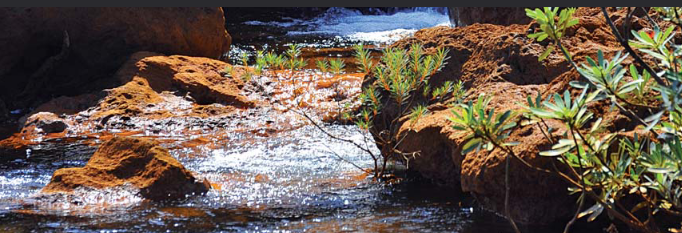
\includegraphics[width=27cm,height=16cm]{../ressources/MJunckerOEIL.jpg}
        };
    \end{tikzpicture}

    %ajout de l'image supérieur
    \begin{tikzpicture}[remember picture, overlay]
        \clip [rounded corners=30pt] (-0.5cm,-2.5cm) rectangle ++(9cm,5.5cm);
        \node[inner sep=0pt, anchor=south west] at (-0.5cm,-2.5cm) { 
            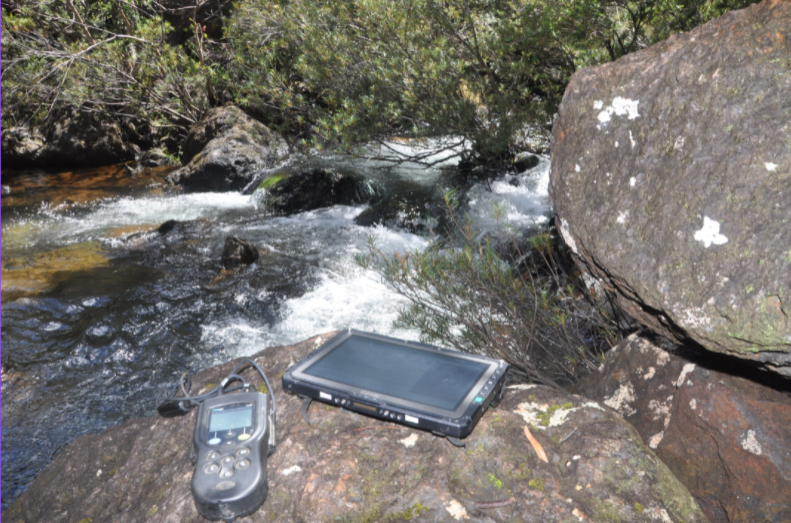
\includegraphics[width=10.5cm,height=6.5cm]{../ressources/eau-monitoring.png}
        };
        \draw [white, line width=3pt, rounded corners=30pt] (-0.5cm,-2.5cm) rectangle ++(9cm,5.5cm); %trait blanc autour de l'image
    \end{tikzpicture}

    %ajout du versionning du rapport
    \begin{minipage}[2cm]{16cm}
        \begin{adjustwidth}{12cm}{1cm} 
            \vspace{0.5cm}
            {\fontsize{10}{12}\selectfont
            \color{version_color}
            
            }
        \end{adjustwidth}
    \end{minipage}

% intégration des titre, sous-titre, auteurs et date
    \begin{minipage}[2cm]{16cm}
        \begin{adjustwidth}{0.5cm}{1cm} 
            \vspace{2.2cm}
            {\fontsize{16}{20}\selectfont
            \color{titreColor}
            \\
            }

            {\fontsize{12}{14}\selectfont
            \color{grey_color}
            Hugo Roussaffa \\
            \\
            }
    
            {\fontsize{12}{8}\selectfont
            \color{date_color}
            2 avril 2026\\
            }

        \end{adjustwidth}
    \end{minipage}

    %ajout du logo OEIL
    \begin{tikzpicture}[remember picture,overlay]
        \node [inner sep=0pt] at (12.5cm,-4.8cm) {\includegraphics[width=4.5cm,height=5.5cm]{../ressources/OEIL\_logo.png} 
        };
    \end{tikzpicture}

    %ajout d'element supplémentaire ou logo partenaire
    \begin{minipage}[1cm]{16cm}
        \begin{adjustwidth}{-0.4cm}{1cm} 
            \vspace{3.4cm}
            \begin{tikzpicture}[remember picture,overlay]
                \node [inner sep=0pt] at (12.5cm,-5cm) {\includegraphics[width=7cm,height=1.5cm]{../ressources/logo\_yapuka.png} 
            };
            \end{tikzpicture}
            {\fontsize{11}{13}\selectfont
            \color{version_color}
            \\ Diffusion Limitée - OEIL/OFB/DAVAR/DASS \\ Nouvelle-Calédonie\\  % ou Logo partenaire/prestataire H, 5.5cm
            }
        \end{adjustwidth}
    \end{minipage}

\end{titlepage}

\renewcommand*\contentsname{Table des matières}
{
\hypersetup{linkcolor=}
\setcounter{tocdepth}{3}
\tableofcontents
}

\section{Contexte et enjeux}\label{contexte-et-enjeux}

\subsection{Contexte externe}\label{contexte-externe}

\subsubsection{État de la menace}\label{uxe9tat-de-la-menace}

Le projet répond à une urgence environnementale marquée par des
pressions et des enjeux multiples :

\begin{itemize}
\tightlist
\item
  \textbf{Incendies} : En 2019, \textbf{17 \% des feux de brousse} ont
  touché des PPE (7 000 hectares);
\item
  \textbf{Érosion} : La couverture végétale est dégradée dans \textbf{90
  \% des PPE} de Nouvelle-Calédonie;
\item
  L'activité minière constitue une pression majeure qui fragilise la
  stabilité des sols et la qualité physico-chimique des eaux en amont
  des prises d'eau.
\item
  \textbf{Changement climatique} : Une baisse de \textbf{20 \% des
  précipitations} est projetée d'ici 2100;
\item
  \textbf{Humain} : La protection de la ressource en eau représente un
  enjeu vital pour \textbf{271 407 habitants} et \textbf{90 800 ménages}
  .
\end{itemize}

\subsubsection{Un cadre réglementaire et institutionnel
nouveau}\label{un-cadre-ruxe9glementaire-et-institutionnel-nouveau}

L'adoption de la loi du pays n° 2025-9 du 15 juillet 2025 relative au
domaine public de l'eau (DPE) et à la protection de la ressource
modernise le cadre juridique calédonien sur la ressource en eau.

L'objectif des PPE est de préserver la qualité de la ressource en
réglementant ou en interdisant les activités polluantes autour des
points de prélèvement, évitant ainsi des frais de traitement onéreux
pour les communes et les usagers.

Le rôle du gouvernement de la Nouvelle-Calédonie ne se limite plus
seulement aux études techniques, il s'étend désormais à la décision
finale de protection.

\paragraph{Adoption de l'arrêté}\label{adoption-de-larruxeatuxe9}

C'est désormais le gouvernement de la Nouvelle-Calédonie qui instaure
par arrêté les périmètres de protection (immédiate, rapprochée et
éventuellement éloignée).

\begin{itemize}
\item
  Instruction centralisée : Le service de l'eau de la DAVAR est confirmé
  comme l'instructeur unique pour les demandes d'autorisation de
  prélèvement et les dossiers de PPE.
\item
  Gestion des urgences : Le gouvernement peut désormais autoriser des
  prélèvements provisoires sans PPE en cas de circonstances climatiques
  exceptionnelles ou de pollution accidentelle, à condition qu'il n'y
  ait pas de danger pour la santé.
\end{itemize}

\paragraph{L'État}\label{luxe9tat}

Alors qu'auparavant l'État signait l'arrêté de Déclaration d'Utilité
Publique (DUP), la nouvelle loi du pays transfère le pouvoir de décision
au gouvernement local :

\begin{itemize}
\tightlist
\item
  Procédure locale : Les modalités de l'enquête publique ne dépendent
  plus des procédures de l'État mais sont désormais fixées par une
  délibération du Congrès (n° 522 du 20 novembre 2025).
\item
  Information : L'État (via le Haut-commissaire) reste informé par la
  transmission des arrêtés et peut être sollicité pour la liste
  d'aptitude des commissaires enquêteurs, mais le pilotage de la
  procédure est calédonien.
\end{itemize}

\paragraph{Les Provinces}\label{les-provinces}

Depuis la rétrocession de la compétence ``eau'' en 2022, leur rôle a
évolué vers le conseil et la concertation :

\begin{itemize}
\tightlist
\item
  Avis obligatoire : Les provinces sont désormais systématiquement
  saisies pour avis lors de l'instruction des dossiers de PPE ou
  d'autorisations de prélèvements importantes.
\item
  Délégation possible : La loi prévoit que le gouvernement peut déléguer
  la gestion du domaine public de l'eau (incluant l'entretien ou la
  délivrance des autorisations) aux provinces via une convention.
\item
  Initiative locale : Elles peuvent demander au gouvernement la création
  de Conseils Locaux de l'Eau (CLE) pour une gestion concertée par
  bassin versant.
\end{itemize}

\paragraph{Les Communes}\label{les-communes}

Leurs responsabilités en matière de distribution d'eau potable
demeurent, mais leur implication dans la procédure de PPE est précisée :

\begin{itemize}
\tightlist
\item
  Consultation systématique : Comme les provinces, les communes doivent
  donner leur avis sur les projets d'installations ou de PPE situés sur
  leur territoire.
\item
  Support de l'enquête publique : Les mairies sont les lieux privilégiés
  pour l'affichage des avis de consultation et la mise à disposition des
  dossiers papier.
\item
  Initiative des CLE : Elles peuvent également être à l'origine de la
  création d'un Conseil Local de l'Eau pour mieux gérer les conflits
  d'usage locaux.
\end{itemize}

\paragraph{Nouveaux échelons et délais
imposés}\label{nouveaux-uxe9chelons-et-duxe9lais-imposuxe9s}

La loi introduit de nouveaux éléments qui n'existaient pas dans le cadre
précédent :

\begin{itemize}
\tightlist
\item
  L'instauration d'un PPE sur terres coutumières est désormais
  strictement conditionnée à l'accord des autorités coutumières,
  matérialisé par un acte coutumier.
\item
  \textbf{Obligation de régularisation} pour les captages existants qui
  n'auraient pas encore de PPE, les gestionnaires disposent d'un délai
  d'un an (à compter du 15 juillet 2025) pour fournir le dossier
  nécessaire à leur détermination.
\item
  Participation du public simplifiée pour les PPE concernant
  \textbf{moins de 12 propriétaires} (et sans impact économique majeur),
  une simple consultation publique de 15 jours remplace la lourde
  procédure d'enquête publique.
\end{itemize}

\subsection{Contexte interne}\label{contexte-interne}

\subsubsection{De PressionPPE à
Hydroscope}\label{de-pressionppe-uxe0-hydroscope}

Le projet Hydroscope succède au tableau de bord \textbf{PressionPPE}
(2021) qui a permis un premier inventaire des données liées à l'eau
potable. Toutefois, ce système a atteint des limites opérationnelles, à
savoir:

\begin{itemize}
\tightlist
\item
  \textbf{Dépendance technique et coûts} : Une forte rigidité liée aux
  solutions propriétaires (ArcGIS) et aux processus manuels SQL/SIG.
\item
  \textbf{Vision temporelle limitée} : l'absence d'historisation et des
  indicateurs non actualisés ne permettent pas de suivre les tendances
  et l'évolution des menaces dans le temps ni d'identifier de
  changements entre 2 dates.
\item
  \textbf{Déficit d'usage} : le tableau de bord a été développé
  spécifiquement pour des spécialistes et l'ergonomie complexe qui
  l'accompagne ne convient pas aux profils des décideurs et du grand
  public.
\end{itemize}

D'autre part, l'application ArcGIS Pro développée en Province Nord pour
le suivi de la ressource en eau potable, qui se limite à ce territoire
et ne répond donc pas aux besoins d'un Système d'Information
Environnemental global pour l'ensemble de la Nouvelle-Calédonie. Cette
application présente néanmoins l'avantage de permettre des calculs
d'indicateurs multicritères pondérés, une fonctionnalité qui devra être
prise en compte dans la conception de la future plateforme Hydroscope.

Il s'agit d'une application uniquement pour les des agents aguerris au
SIG et qui ne permet pas de partage d'information, ainsi que :

\begin{itemize}
\tightlist
\item
  Absence d'automatisation de la collecte et de l'analyse des données;
\item
  Difficulté d'intégration de nouvelles sources de données ou de
  nouveaux indicateurs;
\item
  Dépendance à l'environnement ArcGIS (ArcGIS Server / image, ArcGIS
  Pro);
\item
  Pas d'interfaces adaptées à différents profils d'utilisateurs
  (experts/gestionnaires, partenaires, grand public);
\item
  Absence d'historisation des indicateurs, limitant la capacité à suivre
  les tendances et à analyser les évolutions dans le temps;
\item
  Processus de mise à jour manuel et peu flexible, nécessitant des
  manipulations SQL et SIG, ce qui rend la maintenance et l'évolution du
  système complexes.
\end{itemize}

\subsubsection{Organisation interne et
partenaires}\label{organisation-interne-et-partenaires}

Le projet est porté par l'OEIL, avec le souhait de collaborer avec de
nombreux partenaires, tels que :

\textbf{Les institutions} DAVAR, DASS, DIMENC, Provinces, Communes,
\textbf{Syndicats de gestion de l'eau} (AQUA Nord, SIVOM VKP, CDE),
\textbf{bureaux d'études} (SEREG, GEOS4D, GeoImpact, Bioéco, CAPSE) et
\textbf{associations} (WWF, comité de population locale).

Cette liste de partenaires est priorisée par l'équipe projet puis sera
validée en COPRO.

Le chef de projet MOA identifié à l'OEIL est Marjolaine David, avec un
appui fort de l'AMOA externe (Yapuka - Hugo Roussaffa) pour la tenue des
ateliers, la formalisation du cadrage stratégique, les cadrages
fonctionnels et la rédaction du cahier des charges fonctionnel.

Afin d'appuyer les sollicitations de l'équipe projet auprès des
partenaires lors des ateliers, l'OEIL sollicitera officiellement une
lettre de mission auprès du Gouvernement. Cette démarche vise à
légitimer l'implication des services techniques territoriaux.

\subsubsection{Défis stratégiques et réponses du
projet}\label{duxe9fis-stratuxe9giques-et-ruxe9ponses-du-projet}

\paragraph{Viabilité financière et respect des
jalons}\label{viabilituxe9-financiuxe8re-et-respect-des-jalons}

Le projet repose sur un co-financement OFB (65 \%) et PEP (35 \%), dont
le premier versement est conditionné à la livraison d'un rapport de
critères et fiches indicateurs. Ce jalon constitue une priorité absolue
de la phase de démarrage.

\begin{itemize}
\tightlist
\item
  \textbf{Enjeu} : Garantir la continuité du projet en respectant les
  engagements contractuels envers les financeurs.
\item
  \textbf{Réponse} : Livraison prioritaire du rapport de critères et
  fiches indicateurs, déclenchant le versement de 30 \% du fonds PEP.
\end{itemize}

\paragraph{Connaissance et diagnostic territorial
partagé}\label{connaissance-et-diagnostic-territorial-partaguxe9}

Protéger la ressource en eau potable suppose d'abord de la caractériser
précisément : localisation des bassins versants d'approvisionnement
(BVAEP), périmètres de protection et points de captage, pressions
environnementales associées. Le BVAEP est retenu comme unité de
référence pour l'ensemble du projet --- il constitue le seul périmètre
univoque pour tous les ouvrages et garantit la cohérence des analyses
entre acteurs.

La modélisation structure les relations entre ces trois niveaux
géographiques --- bassin versant, périmètre de protection, captage ---
permettant d'évaluer les pressions de manière cohérente à chaque échelle
et de naviguer entre elles sans rupture d'information.

\begin{itemize}
\tightlist
\item
  \textbf{Enjeu} : Disposer d'un constat commun sur l'état de la
  ressource, utilisable à tous les échelons institutionnels, pour
  orienter les décisions d'investissement et les actions de terrain.
\item
  \textbf{Réponse} : Mise en place d'une analyse multicritère et
  développement de trois interfaces adaptées aux profils des
  utilisateurs (Expert, Partenaire, Grand public), complétées par des
  rapports de synthèse automatisés.
\end{itemize}

\paragraph{Adhésion des utilisateurs et pertinence des
indicateurs}\label{adhuxe9sion-des-utilisateurs-et-pertinence-des-indicateurs}

Un système d'information ne produit de valeur que si ses indicateurs
correspondent aux besoins réels de ceux qui les utilisent, et si l'outil
est suffisamment accessible pour s'intégrer dans les pratiques de
travail. C'est le risque principal du projet : concevoir un système
techniquement solide mais déconnecté des usages, ou trop complexe pour
être adopté durablement.

Cette exigence d'accessibilité doit être intégrée dès la conception ---
dans les choix d'ergonomie, la documentation contextuelle et la capacité
de l'outil à rendre les utilisateurs autonomes sans formation lourde.

\begin{itemize}
\tightlist
\item
  \textbf{Enjeu} : S'assurer que les indicateurs, la modélisation et les
  interfaces répondent aux attentes concrètes des gestionnaires,
  décideurs et experts du territoire, et que l'outil soit approprié par
  ses utilisateurs dans la durée.
\item
  \textbf{Réponse} : Organisation d'un cycle de 6 à 8 ateliers de
  co-construction avec les parties prenantes, permettant de valider
  collectivement les indicateurs, les seuils de vigilance et les choix
  d'interface avant leur développement.
\end{itemize}

\paragraph{Réactivité et veille
environnementale}\label{ruxe9activituxe9-et-veille-environnementale}

Les pressions sur la ressource --- incendies, défrichements, nouvelles
installations --- peuvent évoluer rapidement. Un changement non intégré
et non signalé réduit la capacité des gestionnaires à agir sur les
captages qui sont impactés.

\begin{itemize}
\tightlist
\item
  \textbf{Enjeu} : Réduire le délai entre un événement environnemental
  et son signalement, tout en fiabilisant l'information produite.
\item
  \textbf{Réponse} : Déploiement d'une chaîne de traitement automatisée
  intégrant des algorithmes de détection des changements, assurant une
  veille continue sans intervention manuelle répétitive.
\end{itemize}

\paragraph{Pérennité et indépendance du
système}\label{puxe9rennituxe9-et-induxe9pendance-du-systuxe8me}

Le projet s'inscrit dans la continuité de travaux engagés depuis 2021.
L'enjeu est de consolider ces acquis dans un système durable,
maintenable sans dépendance à des logiciels propriétaires coûteux, et
capable de produire des analyses temporelles sur le temps long.

\begin{itemize}
\tightlist
\item
  \textbf{Enjeu} : Garantir la durabilité du système à coût maîtrisé, en
  évitant la dette technique et en assurant la traçabilité des données
  dans le temps.
\item
  \textbf{Réponse} : Adoption d'un socle open source et mise en place
  d'une historisation réfléchie des données et indicateurs prioritaires,
  avec un cataloguage et une documentation systématiques des procédures.
\end{itemize}




\end{document}
